\documentclass[12pt]{extarticle}
%Some packages I commonly use.
\usepackage[english]{babel}
\usepackage{graphicx}
\usepackage{framed}
\usepackage[normalem]{ulem}
\usepackage{amsmath}
\usepackage{amsthm}
\usepackage{amssymb}
\usepackage{amsfonts}
\usepackage{enumerate}
\usepackage[utf8]{inputenc}
\usepackage{float}
\usepackage{gensymb}
\usepackage[top=1 in,bottom=1in, left=1 in, right=1 in]{geometry}
\usepackage{multirow}
\usepackage{caption}
\usepackage{subcaption}
\usepackage[utf8]{inputenc}

%A bunch of definitions that make my life easier
\newcommand{\matlab}{{\sc Matlab} }
\newcommand{\cvec}[1]{{\mathbf #1}}
\newcommand{\rvec}[1]{\vec{\mathbf #1}}
\newcommand{\ihat}{\hat{\textbf{\i}}}
\newcommand{\jhat}{\hat{\textbf{\j}}}
\newcommand{\khat}{\hat{\textbf{k}}}
\newcommand{\minor}{{\rm minor}}
\newcommand{\trace}{{\rm trace}}
\newcommand{\spn}{{\rm Span}}
\newcommand{\rem}{{\rm rem}}
\newcommand{\ran}{{\rm range}}
\newcommand{\range}{{\rm range}}
\newcommand{\mdiv}{{\rm div}}
\newcommand{\proj}{{\rm proj}}
\newcommand{\R}{\mathbb{R}}
\newcommand{\N}{\mathbb{N}}
\newcommand{\Q}{\mathbb{Q}}
\newcommand{\Z}{\mathbb{Z}}
\newcommand{\grad}{$^{\circ}\:$}
\newcommand{\<}{\langle}
\renewcommand{\>}{\rangle}
\renewcommand{\emptyset}{\varnothing}
\newcommand{\attn}[1]{\textbf{#1}}
\theoremstyle{definition}
\newtheorem{theorem}{Theorem}
\newtheorem{corollary}{Corollary}
\newtheorem*{definition}{Definition}
\newtheorem*{example}{Example}
\newtheorem*{note}{Note}
\newtheorem{exercise}{Exercise}
\newcommand{\bproof}{\bigskip {\bf Proof. }}
\newcommand{\eproof}{\hfill\qedsymbol}
\newcommand{\Disp}{\displaystyle}
\newcommand{\qe}{\hfill\(\bigtriangledown\)}
\setlength{\columnseprule}{1 pt}
\usepackage[utf8]{inputenc}

\title{Imãs, Campo e Força Magnéticas}
\author{Felipe Salvador}
\date{Agosto 2019}

\begin{document}

\maketitle

\section{Introdução}

Começamos o semestre falando de um assunto novo, que é o \textbf{magnetismo}. A gente verá que o magnetismo é um fenômeno um tanto diferente da eletricidade e que ambos, eletricidade e magnetismo, são duas faces de uma mesma moeda, que damos o nome de eletromagnetismo.

Os primeiros estudos de magnetismo são feitos com os \textbf{imãs permanentes.} Esses caras são, em sua maioria, feitos de uma substância chamada de \textbf{magnetita}, que é um dos minérios naturais de ferro. Percebeu-se, lá na Grécia Antiga, que esse minério era atraído e atraía qualquer objeto de ferro.

Os primeiros usos do magnetismo foram feitos pelos chineses na construção de objetos que se assemelhavam a \textbf{bússolas}. Eram colheres feitas de magnetitas, que apoiadas de uma forma que podia rotacionar livremente, sempre apontavam para o Sul. Dessa forma, temos a primeira ideia de uma bússola, que na época de Cabral, foi muito importante para as navegações para África, Ásia e América.

Hoje, após os estudos de Gauss (1777-1855), Ampère (1775-1836), Faraday (1791-1867) e Maxwell (1831-1879), percebeu-se que o magnetismo e a eletricidade eram um mesmo fenômeno, só que 2 formas de se expressar. Esse fenômeno se dá o nome de \textit{eletromagnetismo} e é responsável por 1 das 4 forças naturais.\footnote{As outras 3 são: Gravidade, Força Forte e Força Fraca. As duas últimas são forças nucleares e são responsáveis pela união do núcleo atômico e reações de decaimentos nucleares (como a do urânio), respectivamente.}. Esse fenômeno sozinho explica praticamente tudo que acontece em nós, ao nosso redor, em como nos comunicamos e etc. É o eletromagnetismo que, principalmente, faz acontecer as reações químicas, é possível conectar o celular na internet, faz ser possível esquentar a comida no microondas e muito mais.

\section{Imãs}

O objeto mais simples e comum no magnetismo é o imã. Ele é simples, pois \textbf{o imã possui 2 pólos: o Norte (N) e o Sul (S). Do polo norte (N) sai o Campo Magnético ($\vec{B}$), enquanto no polo sul (S) chega o Campo Magnético ($\vec{B}$)}.

O mais importante sobre imãs é que existe 2 relações sobre pólos:
\begin{itemize}
    \item Pólos iguais se repelem. \textit{Ex: N-N ou S-S};
    \item Pólos diferentes se atraem \textit{Ex: S-N ou N-S};
\end{itemize}

\begin{figure}[h]
    \centering
    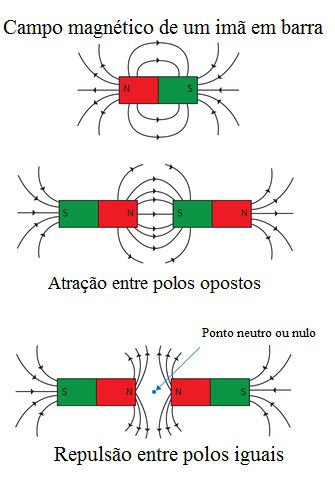
\includegraphics[width=0.4\textwidth]{atracao-repulsao-entre-polos.jpg}
    \caption{De cima para baixo: Diagrama de como é o campo magnético de um imã; como funciona a atração de 2 imãs, em que os polos opostos estão um de frente ao outro; como funciona a repulsão entre 2 imãs, em que os pólos iguais são postos um em frente do outro.}
    \label{fig:atra_repul_ima}
\end{figure}

Temos um nome técnico para quando um objeto magnético, como o imã, tem 2 pólos: \textbf{dipolo}. \textit{Obs: No magnetismo, não é possível obter 1 pólo somente (damos o nome de monopólo).}

Há 2 tipos de imãs:

\begin{itemize}
    \item \textbf{Imã Natural} - são os substâncias/minérios que são encontrados na Natureza e funcionam como imãs. \textit{Ex: Magnetita};
    \item \textbf{Imã Artificial} - são substâncias feitas a partir de metais ou cerâmicos que são submetidos a baíxissimas temperaturas, normalmente, ou a campos magnéticos fortes e apresentam comportamento magnético (atração e repulsão de metais/imãs).
\end{itemize}

A Terra é como um imã gigantesco e é por isso que usamos bússola para nos guiar pelo planeta (até termos o GPS). Porém, o pólo Norte (que fica no Ártico) e o pólo Sul (que fica na Antártida) não são os pólos nortes e Sul de um imã:
\begin{itemize}
    \item Pólo Norte Geográfico $\implies$ pólo sul magnético;
    \item Pólo Sul Geográfico $\implies$ pólo norte magnético.
\end{itemize}

\begin{figure}[h]
    \centering
    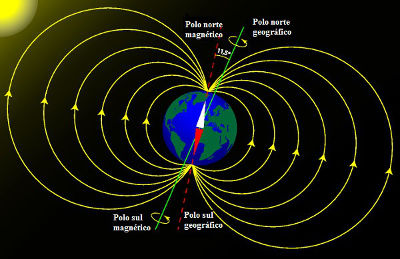
\includegraphics[width=0.5\textwidth]{campo-magnetico-terrestre.jpg}
    \caption{Ilustração de como funciona o campo magnético da Terra, que é devido a Terra ser um imã gigante. Existe uma inclinação de 11,5$^{\circ}\:$ entre eles}
    \label{fig:campo_mag_terra}
\end{figure}

\section{Campo Magnético ($\vec{B}$)}

Até agora falamos de campo magnético sem explicar ao certo o que ele é. \textbf{Um Campo Magnético ($\vec{B}$) é uma grandeza vetorial (pode ser representada por uma flecha) que se refere a concentração de magnetismo, ou seja, a capacidade de atrair/repelir metais e imãs num espaço.}

Um ponto essencial é que \textbf{o campo magnético ele é FECHADO, ou seja, ele começa de um ponto, faz um caminho e termina no mesmo ponto.} Veja que nas figuras anteriores, as linhas e as flechas não vão embora para longe do imã, elas começam e terminam no imã.

A unidade do campo magnético, no SI, é Tesla (T). Nas próximas aulas, iremos ver como é o campo magnético em outros objetos magnéticos.

\section{Força Magnética ($\vec{F}_{mag}$)}

Igual à eletricidade, o campo magnético pode exercer uma força magnética. Só que agora, a força magnética depende da carga elétrica e da velocidade dessa carga elétrica na região do campo magnético. A fórmula dessa força é dada por:
\begin{equation}
    F = |q|.V.B.sin(\theta)
\end{equation}
em que $F$ é a força magnética, $|q|$ é o módulo da carga elétrica, $V$ é a velocidade dessa carga, $B$ é o módulo do campo magnético e $sin(\theta)$ é o ângulo entre a velocidade $V$ e o campo magnético $B$.

\textbf{Um fato importante é que a força magnética é sempre perpendicular à velocidade da carga elétrica e não há força magnética se a carga estiver parada (V=0) ou se o campo magnético ($\vec{B}$) for na mesma direção da velocidade ($\vec{V}$).}

No caso de $\theta = 90^{\circ}$ e carga elétrica positiva ($q>0$), existe uma regra simples para descobrir para onde a força magnética está atuando: \textbf{Regra da Mão Esquerda:}

\begin{figure}[h]
    \centering
    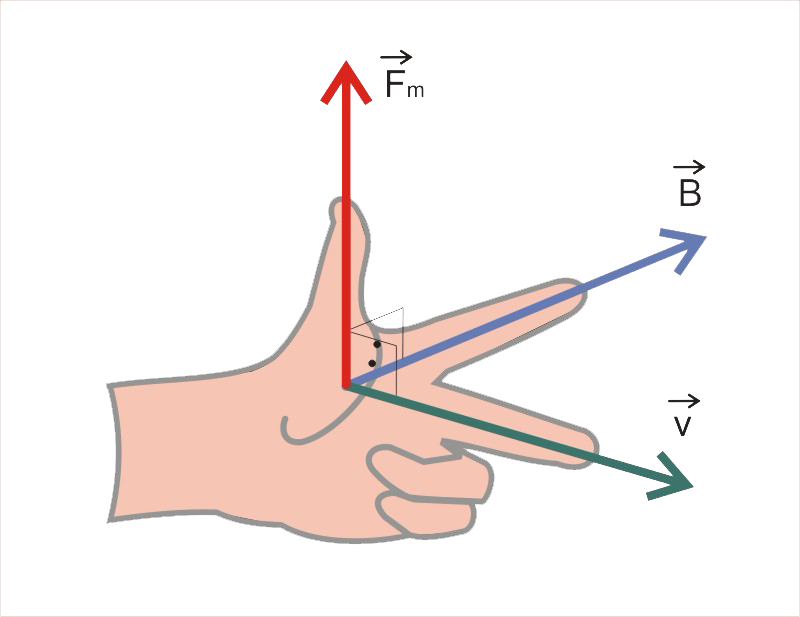
\includegraphics[width=0.5\textwidth]{regra_da_mao_esquerda.png}
    \caption{Ilustração da Regra da Mão Esquerda: o dedo polegar é a direção da força magnética ($\vec{F}$) atua, o dedo indicador é a direção do campo magnético ($\vec{B}$) e o dedo do meio é a direção da velocidade da carga elétrica ($\vec{V}$) }
    \label{fig:regra_mao_esq}
\end{figure}

Para saber a direção da força no caso da carga elétrica positiva, alinhe os dedos do campo magnético e da velocidade com as direções dadas no enunciado e a direção que o dedo polegar indicar é a direção da força. Se a carga for negativa, a direção é a contrária que o dedo polegar indicar.



\textbf{Exemplo 1:} Suponha que uma carga elétrica de 4 $\mu$C seja lançada em um campo magnético uniforme de 8 T. Sendo de 60 \grad o ângulo formado entre v e B, determine a força magnética que atua sobre a carga supondo que a mesma foi lançada com velocidade igual a $5*10^3$ m/s.

Esse exercício é basicamente aplicar os dados na equação da força
\begin{align*}
    F_{mag} &= |q|.V.B.sin(\theta) \\
    F_{mag} &= 4*10^{-6}*5*10^3*8*sin(60^{\circ}) \\
    F_{mag} &= 80*10^{-1} \\
    F_{mag} &= 8 N
\end{align*}

\textbf{Exemplo 2 (PUC):} Um elétron num tubo de raios catódicos está se movendo paralelamente ao eixo do tubo com velocidade $10^7$ m/s. Aplicando-se um campo de indução magnética de 2T, paralelo ao eixo do tubo, a força magnética que atua sobre o elétron vale?
(Dado - carga do elétron: e = $1,6*10^{-19} \:C$)

Como o campo é perpendicular ao movimento do elétron, então $\theta$ = 90\grad. Aplicando a fórmula:
\begin{align*}
    F_{mag}&= |q|.V.B.sin(\theta) \\
    F_{mag} &= 1,6*10^{-19}*10^7*2*1 \\
    F_{mag} &= 3,2*10^{-12} N\\
\end{align*}

Para a força dada acima e sabendo que a massa do elétron é $m_e = 9,1*10^{-31} kg$, calcule a aceleração do elétron.

Para achar a aceleração, vamos usar a Segunda Lei de Newton:
\begin{align*}
    F &= ma \\
    3,2*10^{-12} &= 9,1*10^{-31}.a \\
    a &\approx 1/3 *10^{19} \: m/s^2
\end{align*}

\end{document}
